% WACV 2027 submission — Applications track — ANONYMIZED
% Build with the official WACV 2027 Author Kit (wacv.sty). On Overleaf:
% upload the kit, replace its main.tex with this file, and add references.bib.
% The \usepackage[review]{wacv} line enables the anonymized review layout
% with line numbers and the paper ID header.
\documentclass[10pt,twocolumn,letterpaper]{article}

\usepackage[review]{wacv}      % from the WACV 2027 author kit
\usepackage{times}
\usepackage{graphicx}
\usepackage{amsmath}
\usepackage{amssymb}
\usepackage{booktabs}
\usepackage{multirow}
\usepackage{xcolor}

% Include other packages here, before hyperref.
\usepackage[pagebackref,breaklinks,colorlinks]{hyperref}
\usepackage[capitalize]{cleveref}

\def\wacvPaperID{*****} % *** Enter the Paper ID here
\def\confName{WACV}
\def\confYear{2027}

\begin{document}

%%%%%%%%% TITLE
\title{Evidence-First VLM Cascades for Embedded Work-Zone State Estimation:\\Hyper-Parameter Portability and Out-of-Domain Transfer}

\author{Anonymous WACV submission\\
Paper ID \wacvPaperID}
\maketitle

%%%%%%%%% ABSTRACT
\begin{abstract}
Roadway work zones are dynamic, safety-critical environments commonly addressed with object detectors, semantic verification, and temporal smoothing.  We ask how closely a single work-zone-fine-tuned vision--language model (VLM), quantized to INT4 and running entirely on embedded automotive hardware, can approach such a pipeline while estimating four traversal states (\textsc{outside}, \textsc{approaching}, \textsc{inside}, \textsc{exiting}).  Our \emph{evidence-first cascade} operates one 2B VLM through asymmetric-cost prompt channels and hysteresis, under a \emph{latency-honest} protocol where each system's measured latency determines frame dropping.  On 208 held-out videos it matches a ported detector+CLIP baseline on accuracy and event recall, with a \textsc{approaching}-IoU advantage too small to resolve at this sample size, but trails on precision, nuisance rate, and compute; the gap concentrates in ego-relevance.

A second embedded deployment changes the conclusion.  Applying the 2B model's temporal thresholds to our INT4 4B world-model deployment yields macro-F1 0.290 and \textsc{inside} IoU 0.007; recalibrating the same four integers moves them to 0.515 and 0.574, raising \textsc{inside} IoU by 0.567 absolute.  Thus cross-model comparisons that inherit smoothing constants confound models with hyper-parameters.  On 39 out-of-domain sign approaches spanning night, rain and fog, the fine-tuned 2B detects 5\%, the detector 72\% and the world model 95\%: in-domain results did not predict out-of-domain evidence recovery.  Recalibrated, that deployment is the strongest single system we measure (macro-F1 0.515 vs.\ 0.470), but at twice the detector's false-alarm rate, and the obvious combinations of the two do not resolve the trade-off.  Both VLMs still fail at ego-relevance, indicating an interface rather than checkpoint-specific gap.  These results establish computational viability and experimental competitiveness, not safety readiness; the harness, metrics, prompts, and ported baseline accompany the submission.
\end{abstract}

\begin{figure*}[t]
\centering
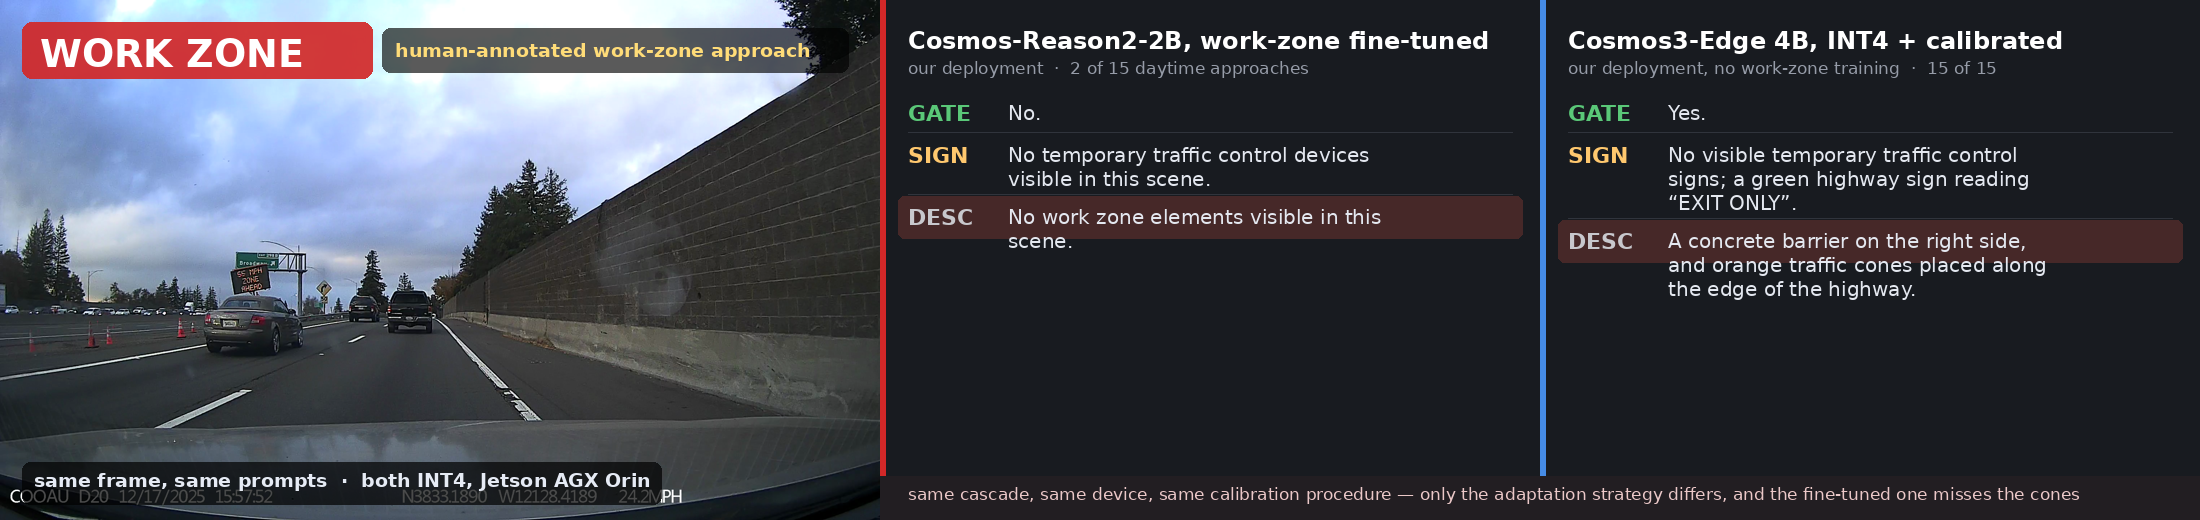
\includegraphics[width=\textwidth]{fig_teaser.png}
\caption{Our two embedded deployments on out-of-domain California footage: the same cascade, Jetson AGX Orin, INT4 recipe, and calibration procedure.  Left: a work-zone-fine-tuned 2B reasoner; right: a zero-shot 4B world model.  Shown are actual greedy on-device replies.  Orange cones cross the left lanes and a concrete barrier borders the right, allowing both outputs to be checked against the image.  Over the 39 approaches of \cref{tab:ood}, the models recover 5\% and 95\%, respectively.}
\label{fig:teaser}
\end{figure*}

%%%%%%%%% BODY TEXT
\section{Introduction}
\label{sec:intro}

Work zones concentrate difficult driving-perception conditions: their appearance is regional and unstandardized, geometry changes daily, evidence such as cones, barrels, signs, and workers is small or occluded, and both misses and nuisance alerts are costly.  They accounted for roughly 101{,}000 U.S. crashes and 899 fatalities in 2023~\cite{nhtsa2023}, yet production ADAS rarely model work zones explicitly and temporary speed limits are often absent from digital maps.

The strongest onboard approach combines a YOLO-style work-zone detector, CLIP verification~\cite{radford2021clip}, exponential smoothing, and hysteresis to estimate four traversal states~\cite{priorsystem2026,priorsystemarxiv2026}.  It is fast and effective after a zone is established, but reported IoU falls from 0.56/0.47 on \textsc{outside}/\textsc{inside} to 0.11/0.09 on \textsc{approaching}/\textsc{exiting}~\cite{priorsystem2026}.  These boundaries are precisely where an advisory is most useful: an alert after the vehicle reaches the barrels has little anticipatory value.

Meanwhile, fine-tuned VLMs describe work-zone scenes well offline~\cite{ghosh2025roadwork}, and weight-only quantization plus embedded runtimes bring small VLMs to automotive hardware~\cite{lin2024awq,trtedgellm}.  We ask whether a single fine-tuned VLM, operated through cooperating prompt channels, can estimate traversal state in real time and compete with the detector pipeline under identical conditions.

Under an identical embedded protocol, the detector-free VLM is competitive on state coverage but trails on precision, nuisance rate, and compute.  Two follow-ups shift the result.  First, temporal thresholds fitted to one checkpoint are not neutral: inherited across models, they move a per-state IoU by $82\times$.  Second, out-of-domain tests show that in-domain results do not predict transfer: a 4B world model we quantize and calibrate, but never fine-tune, recovers 95\% of California work-zone signs versus 5\% for the fine-tuned 2B.  Neither deployment dominates: the world model leads accuracy and boundary localization, the detector leads nuisance and precision.

Answering the original question requires more than swapping models.  At $\sim$10\,ms per output token, a full description costs roughly 500\,ms while a two-token answer costs 75\,ms: prompt choice is an economic decision.  Our cascade exploits three observations (\cref{sec:prompts}): binary prompts are affirmation-biased and resist specialization by rephrasing, so require temporal voting; transcription is faithful and verifiable; and structured descriptions expose disqualifying context such as ``parked'' or ``sidewalk.''  Evidence quality therefore gates smoothing: a transcribed sign can bypass a vote while a binary answer cannot.

Our contributions are: \textbf{(1)} a real-time, fully embedded traversal-state estimator from one quantized VLM; \textbf{(2)} latency-honest evaluation in which measured cycle time drives frame dropping, plus offline per-model recalibration; \textbf{(3)} paired comparison with a carefully reimplemented detector+CLIP port on the same 208 videos, protocol, and device; \textbf{(4)} evidence that temporal hyper-parameters do not transfer between models, with both checkpoints recalibrated symmetrically; \textbf{(5)} a 39-approach out-of-domain benchmark spanning night and weather; and \textbf{(6)} a cross-model analysis of the residual ego-relevance gap.

\section{Related Work}
\label{sec:related}

\paragraph{Work-zone perception.} Early systems used structured environmental models with sensor fusion~\cite{shi2021workzone} or frame-level classification~\cite{abodo2018shrp}.  ROADWork~\cite{ghosh2025roadwork} contains 4{,}375 videos and 9.6K annotated images across 18 U.S.\ cities, and shows that open-vocabulary models improve sharply after in-domain fine-tuning (+32.2 AP for detection and +36.7 SPICE for description).  The closest system~\cite{priorsystem2026} deploys a ROADWork-trained YOLO detector with CLIP verification, EMA smoothing, and hysteresis, and defines the traversal-state evaluation we adopt.

\paragraph{VLMs for driving.} Large VLMs support end-to-end planning~\cite{hwang2024emma,tian2024drivevlm}, open-loop description~\cite{marcu2024lingoqa}, and reasoning~\cite{nvidia2025cosmosreason}, mostly on datacenter GPUs; LightEMMA~\cite{lightemma2025} still targets desktop inference.  We instead estimate one safety-relevant scene state under an embedded latency budget and study prompt-level failures---affirmation bias and distance blindness---that larger models can mask.

\paragraph{World models for physical AI.} Cosmos models jointly learn language, vision, and action for embodied agents~\cite{nvidia2025cosmosreason,nvidia2026cosmos3}; Alpamayo-R1 specializes this recipe for driving with a trajectory decoder and chain-of-causation supervision~\cite{alpamayo2026}.  These systems target planning at datacenter or automotive-SoC scale.  Rather than planning, we quantize a world model for Jetson-class perception, testing whether domain specialization is necessary and whether temporal machinery transfers (\cref{sec:worldmodel}).

\paragraph{Efficient inference and cascades.} AWQ~\cite{lin2024awq} and embedded runtimes~\cite{trtedgellm} enable multi-Hz VLM inference on Orin~\cite{chu2024mobilevlm,lin2024vila}.  Cost-aware cascades are established in classical vision~\cite{viola2001rapid}, video analytics~\cite{kang2017noscope}, and LLM serving~\cite{chen2023frugalgpt,gatekeeper2025}.  Unlike them, our stages share one model: prompts and token budgets create the cost asymmetry, and evidence semantics (transcribed text versus a binary answer), rather than scalar confidence, drive escalation.

\section{System}
\label{sec:system}

\subsection{Two embedded deployments}
\label{sec:deployment}

We deploy \emph{two} models on the same Jetson AGX Orin, adapted in the two ways such a model admits: one by task fine-tuning, one by quantization and per-model calibration alone.  Both run the identical prompt channels, cascade, protocol and splits, so every comparison in this paper varies the model and its adaptation, never the pipeline around it.

\textbf{Fine-tuned 2B.}  A 2B-parameter VLM (Qwen3-VL architecture~\cite{qwen3vl}, initialized from a physical-AI reasoning checkpoint~\cite{nvidia2025cosmosreason}), used for perception only.  We fine-tune it through a ROADWork-derived curriculum~\cite{ghosh2025roadwork}: work-zone VQA ($\sim$46K pairs), ego-state supervision, sign reading, a general-driving retention mix, and $\sim$10K work-zone-free BDD100K hard negatives.  Before the last stage, the existence gate answered ``yes'' on 95\% of clean scenes; after it, 0\% on external negative controls.  Positive-heavy intermediate training had destroyed calibration already present in the base model, and negative examples restored it.  This illustrates why every fine-tuned question type needs both polarities.  Full curriculum and data volumes are in the supplement.

The language backbone is quantized to INT4 (W4A16 AWQ, group size 128), the vision tower stays FP16, and both are compiled to TensorRT engines on-device~\cite{trtedgellm} (1.38\,GB language + 0.83\,GB vision, $\sim$4.5\,GB peak runtime).  A persistent process serves single-image requests.  Costs decompose as 44.6\,ms for vision encoding at 720p or $\sim$20\,ms at 480px, $\sim$0.16\,ms/input token for prefill, and 10.4\,ms/output token for decoding.  Output length therefore dominates, followed by input resolution; 480px preserved probe answers while saving 45\,ms/cycle.

\textbf{Quantized 4B world model.}  Cosmos3-Edge (C3E)~\cite{nvidia2026cosmos3} is a 4B physical-AI world model pairing an autoregressive reasoner with a trajectory-generating diffusion transformer.  We quantize its reasoner to W4A16 AWQ INT4 (1.27\,GB) and keep its visual tower in FP16 (983\,MB), both as TensorRT engines on the same Orin; its frozen $26{\times}46$ patch grid fixes inputs at $736{\times}416$, and channel latencies are 162/182/488/556\,ms (\textsc{gate}/\textsc{ego}/\textsc{desc}/\textsc{sign}).  It receives no work-zone training data and has never seen this benchmark.  Building its engines required six patches to the embedded runtime; that patch set, and the full deployment recipe, are in the supplement.

\subsection{Prompt channels and their failure modes}
\label{sec:prompts}

We operate four fixed-prompt channels with fixed token budgets.  Because the first generated token is an answer-start token, the minimum useful budget is two tokens.


\paragraph{Affirmation bias.} The \textsc{gate} asks a neutral existence question and is calibrated on clean scenes, but binary prompts cannot be specialized by rephrasing.  Variants asking whether work affects the vehicle's path all answered ``yes'' on \textsc{outside} probes, while distance prompts answered ``close'' regardless of scene.  The learned discrimination resides in the trained question; prompt nuance does not transfer.  Binary outputs are therefore weak evidence requiring a temporal vote, never sole triggers.

\paragraph{Faithful transcription.} The \textsc{sign} channel returns stable, verbatim text such as ``\textsc{shoulder work}'' and correctly reports absence.  A binary rephrasing misses signs that transcription catches on the same frames.  We therefore transcribe and derive a binary value by matching a work-zone keyword lexicon.

\paragraph{Structured corroboration.} The \textsc{desc} channel's object--location prefix often verbalizes disqualifying context---e.g., ``barriers on right \emph{sidewalk}'' or ``work vehicle \emph{parked}.''  Corroboration therefore requires a work-zone object without such a qualifier.  Byte-exact prompts, budgets, and lexicons are in the supplement.

\subsection{Evidence-first cascade}
\label{sec:cascade}

\begin{figure}[t]
\centering
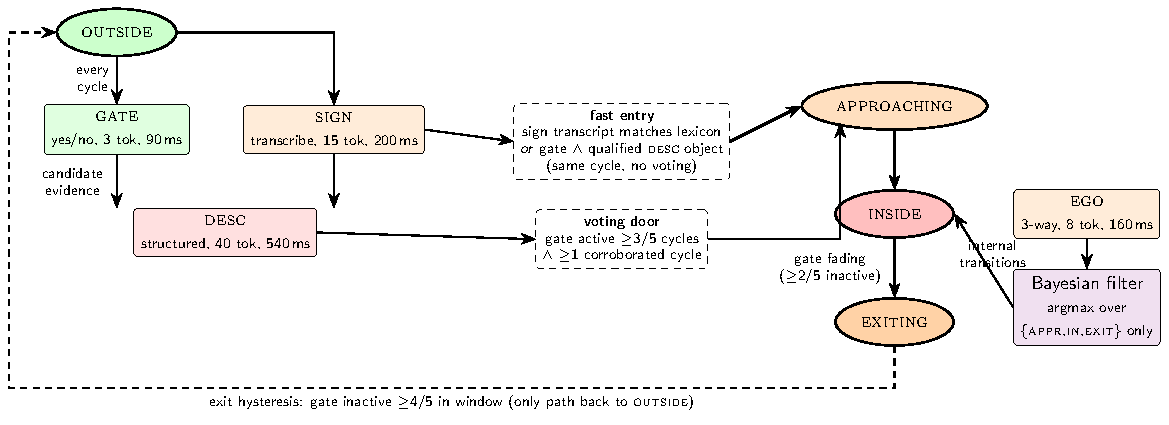
\includegraphics[width=\linewidth]{fig_cascade.pdf}
\caption{Evidence-first cascade.  In \textsc{outside}, \textsc{gate} and \textsc{sign} run every cycle and candidate evidence invokes \textsc{desc}.  Entry requires a sustained, corroborated vote or high-confidence same-cycle evidence.  In active states, \textsc{ego} drives a Bayesian filter; sustained gate clearance returns to \textsc{outside}, while partial fading triggers \textsc{exiting}.  Constants are calibrated per model: $5/3/4/2$ for the 2B and $3/3/2/1$ for C3E, so the structure transfers but the numbers do not.}
\label{fig:cascade}
\end{figure}

The cascade (\cref{fig:cascade}) allocates compute by state.

\textbf{Outside (patrol).}  \textsc{gate} and \textsc{sign} run every cycle ($\sim$315\,ms, 3.2\,Hz); either can invoke \textsc{desc}.  Entry into \textsc{approaching} has two paths: a voting path, with the gate active in at least three of five cycles and one corroboration, or fast entry on a lexicon-matching sign or gate+\textsc{desc} agreement in the same cycle.  Fast entry avoids the $\sim$1.6\,s voting delay for evidence such as a transcribed ``\textsc{road work ahead}.''

\textbf{Active states.}  \textsc{ego} updates a Bayesian filter whose argmax is restricted to the three active states.  Otherwise, a single ``outside'' reply immediately after sign-triggered entry would erase the sign's anticipatory value.  Only sustained gate clearance returns the system to \textsc{outside}; partial fading triggers \textsc{exiting}, which \textsc{ego} never produced even when offered explicitly.  \textsc{desc} refreshes every 1.5\,s.  All thresholds ($N{=}5$, $K_\text{enter}{=}3$, $K_\text{exit}{=}4$, $K_\text{fade}{=}2$) were fixed on calibration data.

These asymmetries encode evidence quality rather than model confidence.  A sign transcription provides discrete, externally checkable evidence and can trigger fast entry; a binary answer is cheap but must survive voting; a description is expensive and therefore conditional.  Likewise, state exit is assigned to sustained disappearance rather than a single language reply.  The design lets the VLM spend tokens where their semantics justify the latency, while hysteresis absorbs the known failure modes of short answers.



\section{Evaluation Protocol}
\label{sec:protocol}

\paragraph{Benchmark.} We use the detector baseline's 520-video ROADWork-derived traversal benchmark~\cite{priorsystem2026}: Boston and Seattle footage at 1920$\times$1080, 30\,fps, with 484K interval-labeled frames.  A state-stratified 60/40 video split assigns all design choices and thresholds to calibration (312 videos, 2.59\,h) and final results to validation (208 videos; 192{,}135 frames, 1.78\,h, 13 pure-negative videos); the benchmark totals 4.37\,h of annotated driving.  All systems see the same split.  All 25 drives occur in both partitions, so they are not route-independent (\cref{sec:limitations}).  Interval labels are evaluation-only and hard negatives come from BDD100K.  Fine-tuning images and benchmark videos both derive from ROADWork, so depicted-zone overlap is possible; the ROADWork-trained baseline shares this condition.

Calibration and validation agree within 0.1--1.5 points across primary aggregates.  This argues against threshold overfitting to calibration videos, but not for route or geographic generalization.  A video-level split within shared drives is weaker than a drive-disjoint split even when adequate for choosing state-machine constants.

\paragraph{Latency-honest camera simulation.} Embedded perception cannot pause the world.  After each measured inference cycle of duration $\Delta$ on the target hardware, the replay advances by $\Delta$ and drops intervening frames exactly as a live camera would.  Slower systems therefore observe fewer, sparser frames and pay latency inside the accuracy result rather than beside it.  Predictions are held between cycles, matching a driver-facing display, and scored per frame.

This prevents a heavyweight model from inspecting every frame of a 30\,fps video and reporting latency separately as though accuracy were unchanged.  Each branch's realized latency determines the next frame, so expensive evidence escalation has the same observation cost it would have online.

\paragraph{Metrics.} We adopt the baseline's suite~\cite{priorsystem2026}: frame accuracy and macro-F1; per-state IoU; event precision/recall, where an interval is correct if it overlaps one of the same state; matched-event entry offset; and transition matching at $\pm\{0,5,15,30\}$ frames.  Videos beginning in a state contribute no entry event.  Event metrics capture whether the warning occurs at all, whereas IoU and timing capture boundary quality; both are needed because a long, early interval can have perfect recall but poor localization.  Confidence intervals and paired tests use 10{,}000 video-level bootstrap samples, resampling the same video indices for paired systems; details are in the supplement.

\section{Results: One Fine-Tuned Model vs.\ the Detector}
\label{sec:results}

\subsection{Comparison with the deployed detector system}
\label{sec:vsdetector}

\begin{table}[t]
\centering
\footnotesize
\setlength{\tabcolsep}{1.9pt}
\begin{tabular}{@{}lccccc@{}}
\toprule
& \multicolumn{2}{c}{Detector+CLIP~\cite{priorsystem2026}} & \multicolumn{2}{c}{\emph{ours}: 2B{+}FT} & \emph{ours} \\
\cmidrule(lr){2-3}\cmidrule(lr){4-5}\cmidrule(lr){6-6}
Metric & pair & {+}FE & raw & rec.\ & C3E \\
\midrule
Frame acc.\ & 62.9\% & 62.9\% & 62.5\% & 62.0\% & \textbf{65.5\%} \\
Macro F1 & 0.470 & 0.473 & 0.464 & 0.453 & \textbf{0.515} \\
\midrule
IoU \textsc{out} & \textbf{0.617} & 0.594 & 0.586 & 0.581 & 0.615 \\
IoU \textsc{appr} & 0.124 & 0.140 & 0.152 & 0.152 & \textbf{0.278} \\
IoU \textsc{in} & 0.544 & 0.555 & 0.535 & 0.532 & \textbf{0.574} \\
IoU \textsc{exit} & \textbf{0.106} & 0.104 & 0.085 & 0.062 & 0.071 \\
\midrule
\textsc{in} ev.\ recall & 95.7 & 95.1 & \textbf{96.8} & 96.8 & 87.0 \\
\textsc{in} ev.\ prec.\ & 79.9 & \textbf{81.9} & 54.1 & 76.7 & 71.5 \\
False alarms/h & \textbf{30.9} & 52.3 & 60.1 & 37.7 & 64.6 \\
\midrule
Entry MAE & 2.52 & 2.42 & 2.53 & 2.52 & \textbf{2.15} \\
Entry med.\ & 1.37 & 1.45 & 1.37 & \textbf{1.27} & 1.37 \\
\textsc{in} entry med.\ & 3.47 & 3.05 & 2.73 & 2.77 & \textbf{2.50} \\
\bottomrule
\end{tabular}
\caption{Validation split, 208 videos, all systems under one protocol (event P/R in \%, timing in s).  The external baseline comes first; the three right-hand columns are our two deployments (\cref{sec:deployment}), which differ in how the model was adapted, not in who built the pipeline around it.  \emph{pair}: our port of the detector+CLIP pipeline; \emph{{+}FE}: that detector with the VLM's text fast entry; \emph{raw}: the cascade of \cref{sec:cascade}, sampled decoding; \emph{rec.}: greedy plus a 1\,s \textsc{inside} debounce; \emph{C3E}: the world-model deployment with its own calibrated thresholds.  Both VLM columns use the published thresholds; recalibrating them symmetrically (\cref{sec:worldmodel}) moves the 2B only 0.453$\to$0.459, so this is not a handicap.  No configuration dominates: C3E leads accuracy, macro-F1 and both boundary IoUs, the detector leads nuisance and \textsc{inside} precision.}
\label{tab:main}
\end{table}

\Cref{tab:main} places every system on the same videos, device and protocol.  This section reads its left four columns---the question the paper set out to answer, one fine-tuned model against the deployed detector; the two world-model columns are the outcome of \cref{sec:worldmodel} and are discussed there.  Against the ported detector+CLIP pair, the fine-tuned 2B is statistically tied on frame accuracy and \textsc{inside} event recall, and shows a small \textsc{approaching}-IoU advantage (0.152 vs.\ 0.124) whose paired 95\% CI marginally includes zero ($[-0.005,+0.058]$, 10{,}000 video-level replications), but trails badly on event precision (54.1\% vs.\ 79.9\%).  This is a competitive detector-free result rather than a replacement result.  Greedy decoding plus a 1\,s \textsc{inside} debounce recovers most of the precision gap (76.7\%) without retraining, at a small cost in boundary IoU.  Median entry error is comparable across systems (1.27\,s for the debounced 2B against 1.37\,s for the detector), while the 2B's \textsc{inside} entry median is better by 0.70\,s.

Grafting the VLM's text fast entry onto the detector (\emph{{+}FE}) improves \textsc{inside} IoU (0.544$\to$0.555), precision (79.9\%$\to$81.9\%) and mean entry error, showing that the transcription channel carries evidence the detector lacks.  It also raises false alarms from 30.9 to 52.3/h, because that evidence enters through the detector's own smoothing and can open its state machine on a single reading.

We omit the baseline's published macro-F1 of 0.60 from the table: it uses a different split and does not apply latency-honest frame dropping, so it is not directly comparable to any column here (\cref{sec:limitations}).

The four-state pattern matters more than aggregate accuracy.  Both learned pipelines perform well on established \textsc{inside} intervals but poorly on \textsc{exiting}; the VLM's main advantage is \textsc{approaching}, where text and distant semantic evidence appear before detector counts become stable.  Conversely, the detector's stronger \textsc{outside} IoU and lower nuisance rate show why semantic anticipation cannot be accepted unconditionally.  This state-wise complementarity, rather than a small difference in overall accuracy, is the result that survives.

Transition-tolerance results in the supplement agree: relaxing the matching window recovers entries for every system without reordering them, so the anticipation advantage is not an artifact of exact frame alignment, and the detector's precision advantage persists under event scoring, so the VLM's nuisance problem is not merely shifted boundaries.

\begin{figure*}[t]
\centering
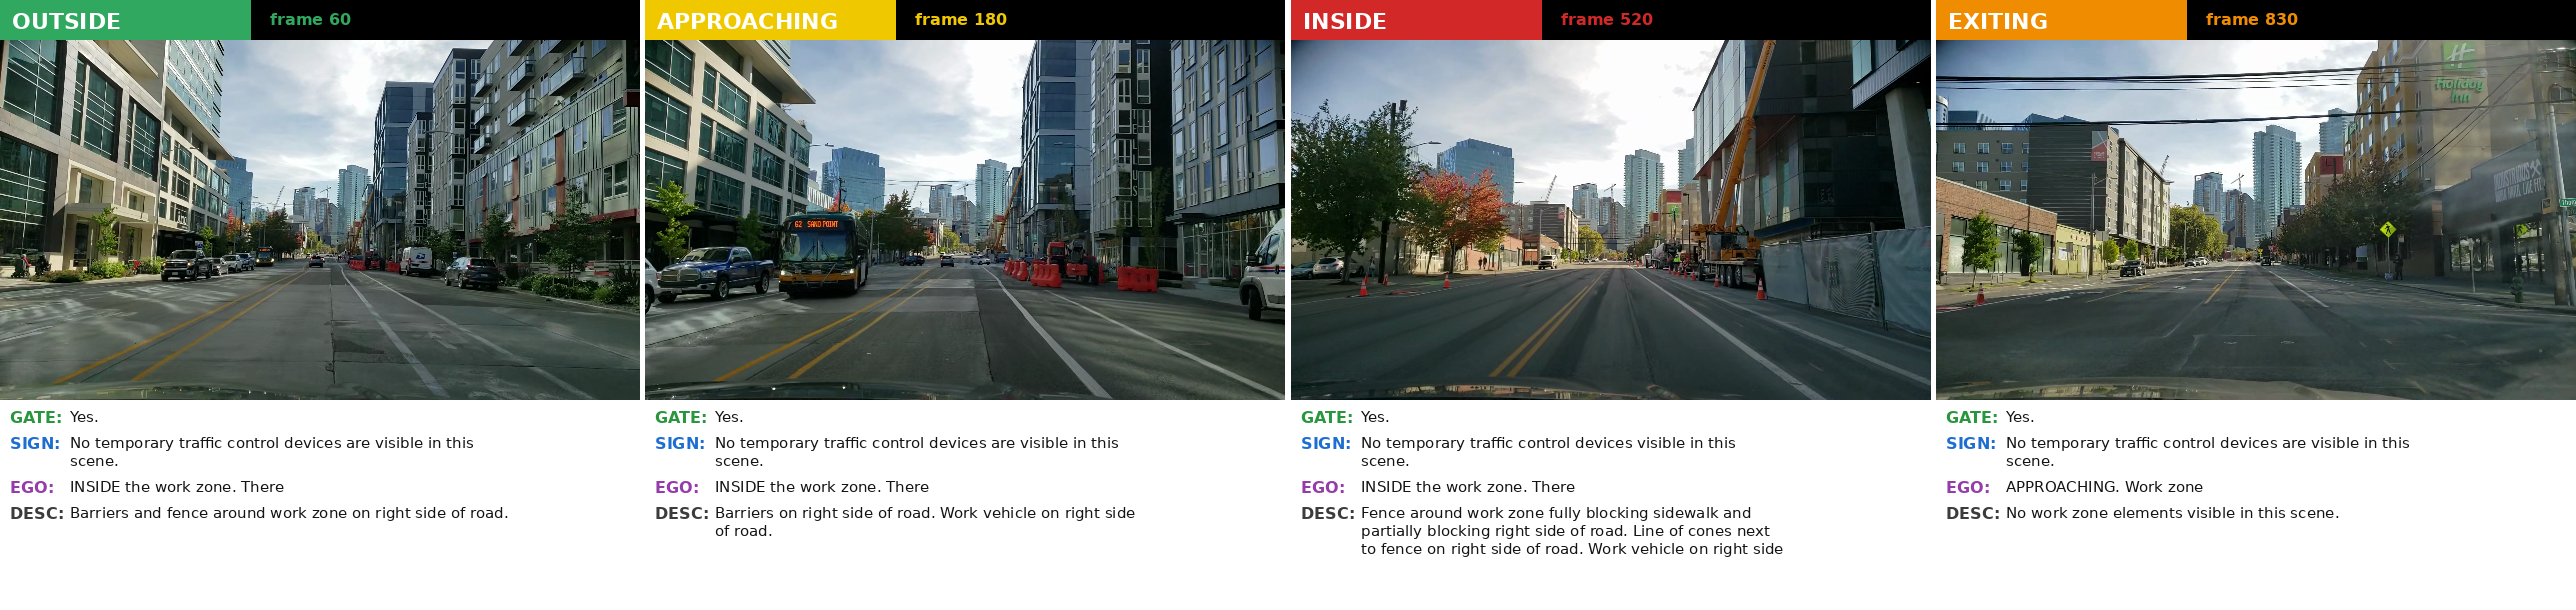
\includegraphics[width=\textwidth]{fig_qualitative.png}
\caption{One continuous validation traversal (Seattle; ground-truth state colored in each banner), with the \emph{actual} per-channel VLM outputs below each frame.  \textsc{outside}: the vehicle has not yet reached the zone, but \textsc{gate} and \textsc{desc} already register the barriers down the block (and \textsc{ego} over-fires ``inside'')---the anticipatory early detection the paper quantifies, and a first illustration of why no single channel is trusted alone.  \textsc{approaching}: barriers and a work vehicle enter the frame; \textsc{gate}+\textsc{desc} corroborate. \textsc{inside}: the vehicle is amid cones and a crane truck, with \textsc{desc} naming the fence and cone line.  \textsc{exiting}: objects recede, \textsc{gate} begins to fade and \textsc{ego} drops back to ``approaching''---the partial-fading trigger---before exit hysteresis returns the state to \textsc{outside}.  \textsc{desc} is truncated to its object--location prefix, the only part the cascade consumes.}
\label{fig:qualitative}
\end{figure*}

\subsection{Operational false-alarm characterization}
\label{sec:falsealarms}

A driver-facing system is judged by nuisance rate, not only event precision.  Over 1.78\,h, false active-state events occur at 60.1/h; greedy plus 1\,s debounce cuts this to 37.7/h (2\,s: 27.5/h), versus 30.9/h for the detector.  Specificity is measured on 75{,}918 \textsc{outside} frames (70.6\% correctly held) and on all 36 pure-negative videos (13 validation, 23 calibration), where the system remains \textsc{outside} for 67.4\% and 58.0\% of their frames respectively.  Residual errors are predominantly the ego-relevance family of \cref{sec:analysis}, not clean-scene noise.  Of 155 matched \textsc{inside} entries, 81.9\% fire early relative to the interval annotation (median 2.4\,s)---the preferable direction for an advisory, though earliness is not itself a safety argument once nuisance is counted--- but anticipation stretches intervals and lowers event temporal IoU (mean 0.263; stricter thresholds are reported in the supplement).

Debounce therefore exposes a genuine operating point rather than a universally superior setting: longer persistence suppresses nuisance but delays or removes short valid events.  We report the raw and recommended settings rather than hiding this trade-off behind one selected number.

\subsection{Ablations and design validation}
\label{sec:ablations}

Seven single-toggle ablations (full table and per-toggle discussion in the supplement) show that no component moves frame accuracy or macro-F1 by more than 1.5 points, yet each protects a targeted failure.  The sign channel must transcribe rather than classify: an equal-cost binary question is the most damaging change, reducing accuracy 62.5\%$\to$52.5\% and \textsc{inside} precision to 46.1\%.  The binary form answers ``yes'' to signage in general while missing signs that transcription reads correctly on the same frames.  Removing the channel barely moves aggregates because its value is anticipatory entry rather than frame correctness---the behaviour \cref{fig:qualitative} traces frame by frame.  Greedy decoding costs 0.5 accuracy points but improves precision at matched recall, making it our reproducible default.  Fast entry, qualifier filtering, and active-state filtering protect behaviors poorly captured by aggregate metrics; the qualifier filter is largest, adding 2.2 points concentrated in pure-negative videos.

\paragraph{Does fine-tuning do the work?}  With the base checkpoint, \textsc{inside} IoU falls 0.535$\to$0.012 and recall 96.8\%$\to$0.5\%, suggesting that fine-tuning rather than prompting creates the behavior.  But this control swaps the checkpoint while retaining thresholds fitted to the fine-tuned model, so it measures the pair, not the model.  \Cref{sec:worldmodel} separates the two factors by recalibrating both checkpoints independently; the conclusion survives, but at roughly half the apparent size.

The remaining toggles validate the cascade's asymmetries.  Removing fast entry delays warnings without materially changing dominant \textsc{inside} frames; allowing the Bayesian filter to return directly to \textsc{outside} makes sign-triggered entries collapse before cones become visible; and removing qualifier filtering concentrates errors in scenes containing real but irrelevant construction.  These effects explain why aggregate ablations look small even though the operational behaviors are distinct.

\subsection{Operational cost and cross-city consistency}
\label{sec:cost}

At 480px, p50/p95 latency is 83/90\,ms (\textsc{gate}), 136/149\,ms (\textsc{ego}), 155/169\,ms (\textsc{sign}), and 468/508\,ms (\textsc{desc}).  Patrol and active cycles run at p95 259\,ms (3.9\,Hz) and 239\,ms (4.2\,Hz); the heaviest path is 768\,ms (1.3\,Hz).  Here ``real time'' means keeping pace with a live camera at these rates, not meeting a specific alert deadline.  Under load, the VLM draws 36.5\,W median (42.5\,W peak; 7.9\,W idle) and 3--26\,J/cycle, versus $\sim$24\,W and $\sim$1\,J for the 43\,ms detector: $1.5\times$ the power and $3$--$26\times$ the energy per decision.  Each channel currently re-encodes the frame; sharing its visual embedding is an obvious route to reduce the gap.  Accuracy is stable across Boston/Seattle for both VLM (61.2/66.3\%) and detector (63.3/61.7\%), but stability within one dataset does not establish geographic generalization.

\section{Varying the Model: Calibration and Generalization}
\label{sec:worldmodel}

\Cref{sec:results} held the model fixed while varying its pipeline, confounding the checkpoint with thresholds fitted to it.  The base-checkpoint ablation changes only the former and appears to settle the question, but inherits the latter.  We separate the two factors using the second deployment of \cref{sec:deployment}, recalibrating each checkpoint on its own evidence.  This changes two conclusions above and produces our strongest system.

\paragraph{Temporal hyper-parameters do not transfer.}  With the 2B thresholds, C3E scores macro-F1 0.290 and \textsc{inside} IoU 0.007 at 3.8\% recall.  Taken literally, this would mean that C3E cannot recognize being inside a zone.  It is an artifact.  Recalibrating the same four integers for C3E moves these to 0.515, 0.574, and 87.0\% on validation: \textsc{inside} IoU rises 0.567 absolute and recall 83.2 points, with model, prompts and videos fixed (\cref{tab:worldmodel}); the $82\times$ ratio is large mainly because the inherited value is near zero.  The search covers $N\in\{3,5,7,9\}$, $K_\ast\in 1..N$ and the \textsc{ego}/\textsc{sign} switches (4{,}896 configurations), scored by calibration macro-F1.  The selected configuration ($N{=}3$, $K_{\text{enter}}{=}3$, $K_{\text{exit}}{=}2$, $K_{\text{fade}}{=}1$) is shorter and less hysteretic, consistent with less noisy per-frame evidence, and disables \textsc{ego} (\cref{sec:analysis}).

This is a reusable methodological point: inherited smoothing constants turn model comparisons into comparisons with another model's hyper-parameters.  We make per-model recalibration cheap by recording each channel's output once per sampled frame and replaying the state machine, reducing a threshold sweep from GPU-hours per configuration to CPU-seconds.

Replay does not alter language outputs or select favorable frames; it evaluates only temporal logic over a fixed record.  We ran the identical search on the identical calibration videos for the fine-tuned 2B as well.  It prefers the same shorter window but, unlike C3E, keeps \textsc{ego} enabled, and recalibration buys it little on validation: macro-F1 0.453$\to$0.459, against 0.290$\to$0.515 for C3E.  That asymmetry is the point---a search merely rewarding flexibility would have helped both equally, whereas this one barely moves the model its thresholds were fitted to and transforms the one that inherited them.

The same procedure also settles the fine-tuning question of \cref{sec:ablations} under matched conditions.  Recalibrating the \emph{base} checkpoint---identical family, scale, architecture and visual tower, differing only in the work-zone curriculum---lifts it from macro-F1 0.281 to 0.383 on calibration, against 0.451 to 0.496 for the fine-tuned version.  Given their own thresholds, fine-tuning is worth $+0.113$ macro-F1 and $+8.8$ accuracy points, not the near-total collapse the uncalibrated control implies.  It buys a real and specific capability in domain; \cref{tab:ood} is what it costs outside.  Thus the $82\times$ change isolates fitting the wrapper to its model rather than extra visual training or validation leakage.

\begin{table}[t]
\centering
\footnotesize
\setlength{\tabcolsep}{3pt}
\begin{tabular}{@{}lcccc@{}}
\toprule
& \multicolumn{2}{c}{best of \cref{tab:main}} & \multicolumn{2}{c}{C3E (ours, no FT)} \\
\cmidrule(lr){2-3}\cmidrule(lr){4-5}
Metric & 2B rec.\ & det.\ pair & inherited & calibrated \\
\midrule
Frame acc.\ & 62.0\% & 62.9\% & 43.6\% & \textbf{65.5\%} \\
Macro F1 & 0.453 & 0.470 & 0.290 & \textbf{0.515} \\
IoU \textsc{appr} & 0.152 & 0.124 & 0.233 & \textbf{0.278} \\
IoU \textsc{in} & 0.532 & 0.544 & 0.007 & \textbf{0.574} \\
\textsc{in} ev.\ recall & \textbf{96.8} & 95.7 & 3.8 & 87.0 \\
\textsc{in} ev.\ prec.\ & 76.7 & \textbf{79.9} & 38.9 & 71.5 \\
False alarms/h & 37.7 & \textbf{30.9} & 46.1 & 64.6 \\
\bottomrule
\end{tabular}
\caption{Same C3E model, prompts, and 208 videos; only four window constants differ.  \emph{inherited} uses 2B thresholds; \emph{calibrated} fits them for C3E on calibration data.  Recalibration raises \textsc{inside} IoU $82\times$ and leads on accuracy, macro-F1, and both shown IoUs, but has the worst nuisance rate---motivating the detector gate.}
\label{tab:worldmodel}
\end{table}

\Cref{tab:worldmodel} holds the visual inputs, prompts, model weights, and validation videos fixed.  The inherited configuration would support the substantive but false conclusion that C3E cannot recognize \textsc{inside}; calibration instead makes it the strongest single model on frame accuracy, macro-F1, and the two central IoUs.  The cost is also clear: fewer votes preserve its boundary evidence but expose its affirmative gate, producing the highest false-alarm rate.  Per-model calibration is therefore necessary for validity but does not remove the need to report nuisance behavior.

Notably, calibration disables the \textsc{ego} channel entirely.  A seemingly task-specific question can thus reduce end-to-end accuracy even for a physical-AI world model; the cascade performs better when direct evidence and temporal structure infer state.  This reinforces that prompt availability is not evidence of prompt reliability, and that channel selection must be calibrated alongside window constants.

\paragraph{Out-of-domain generalization.}  We recorded 48.7\,min of continuous California driving across 14 dashcam videos (median 2.2\,min, longest 9.0\,min) with a different camera and conditions absent from the benchmark, then annotated every work-zone sign approach in them---39 in total, spanning daylight, sunset, night, rain and fog (\cref{tab:ood}).  The count is small because it is exhaustive over this footage, not sampled from it.  Annotation and scoring details are in the supplement.

\begin{table}[t]
\centering
\footnotesize
\setlength{\tabcolsep}{3.5pt}
\begin{tabular}{@{}lcccccc@{}}
\toprule
 & all & day & eve+sun & night & rain & fog \\
 & (39) & (15) & (6) & (9) & (4) & (5) \\
\midrule
2B, fine-tuned & 5\% & 13\% & 0\% & 0\% & 0\% & 0\% \\
detector+CLIP & 72\% & 93\% & \textbf{100\%} & 44\% & 50\% & 40\% \\
C3E, calibrated & \textbf{95\%} & \textbf{100\%} & \textbf{100\%} & \textbf{100\%} & \textbf{75\%} & \textbf{80\%} \\
\bottomrule
\end{tabular}
\caption{Detection on 39 hand-annotated California sign approaches.  A detection is a \textsc{gate} activation or work-zone keyword transcription anywhere in the 6\,s approach; all systems share the window and rule, giving a paired per-sign comparison.}
\label{tab:ood}
\end{table}

The fine-tuned model recovers 5\% and zero outside daylight---it does not merely degrade off distribution but fails in every non-day condition.  The detector reaches 72\%, retaining daylight while losing roughly half its recall at night and in weather.  C3E reaches 95\%, perfect through night and missing only rain and fog approaches where signs are often physically illegible, despite never seeing a work-zone training example.

The benchmark deliberately scores the earliest shared capability rather than four-state estimation: one 6\,s window per approach, counting gate activation or sign-keyword transcription, paired across systems.  It isolates whether relevant evidence is perceived under domain shift.  Per-condition cells are descriptive---four rain and five fog approaches cannot support a weather-robustness claim---but the ordering is not: outcomes are perfectly nested across the 36 signs all three systems score, so exact paired McNemar tests give $p=0.016$ (C3E over the detector), $p=6\times10^{-8}$ (detector over the fine-tuned 2B) and $p=5\times10^{-10}$ (C3E over the 2B), with no discordant sign in the opposite direction.  We therefore state the conclusion narrowly, because the two deployments differ in scale, family, pretraining and visual tower as well as in specialization: \emph{in-domain result did not predict out-of-domain evidence recovery here}.  We cannot attribute the gap to fine-tuning alone, and 39 approaches cannot establish that non-specialized models generally win.  What the experiment does show is operational---reporting only ROADWork validation would have selected the wrong perception model for our own footage.

Every decision in this paper is made on the 312-video calibration partition and none on validation: prompts, budgets and the qualifier lexicon on the full partition, and per-model thresholds by replaying recorded evidence over a 100-video subset of it.  The 208 validation videos enter only as the reported result.

\paragraph{No configuration dominates.}  The two deployments fail complementarily: C3E leads accuracy, macro-F1 and both boundary IoUs, but at 64.6 false alarms/h against the detector's 30.9; the detector leads nuisance and \textsc{inside} precision but localizes boundaries poorly.  We report both rather than a single recommendation, because the choice depends on whether an application can absorb a doubled nuisance rate for better boundaries.  \Cref{sec:limitations} records the combinations we tried and why they did not resolve the trade-off.

\paragraph{Trajectory generation is not yet real-time.}  C3E reconstructs 6\,s of ego motion within 1--4\% of the recordings' GPS, but needs 8.8--20.8\,s per tick on Orin against a 6\,s control budget.  TensorRT export is blocked by a 5.9\,GB transformer exceeding ONNX's 2\,GB protobuf limit.  We report a capability validated on this hardware, not a deployed component.

\section{Failure Analysis: the Ego-Relevance Gap}
\label{sec:analysis}

Nearly all residual false-positive mass has one signature: descriptions are factually correct about objects irrelevant to the vehicle's path.  Examples include a parked work vehicle more than 60\,m away, sidewalk reconstruction behind barriers, and residual detour signs for another street.  The qualifier filter catches only cases where the model verbalizes this context; it does not emit qualifiers reliably, and binary or distance prompts do not recover the judgment.

The natural reading is incomplete fine-tuning coverage: empty hard negatives do not teach that visible work-zone objects can be irrelevant.  A control shows that this is not the whole explanation.  C3E transcribes signs correctly, emits plausible 2D boxes, and generalizes where our 2B fails, yet labels most verified \textsc{inside} frames ``off-road/sidewalk'' in ego-lane probes, nearly independently of ground truth.  It exhibits the same failure with the same sign as the fine-tuned model.  Geometric prompting also fails: an ego corridor built from the model's own boxes inherits the query's affirmation bias, because ``locate all work-zone objects'' presupposes their existence and produces boxes in 6/6 pure-negative probes.  Geometry cannot correct bias in its own input.

The comparison is important because C3E is not globally weak on these scenes: it is the strongest model after calibration and dominates out of domain.  Its failure on ego-relevance therefore cannot be dismissed as missed perception, insufficient parameter count, or one positive-heavy fine-tuning run.  Both models can say \emph{what} is visible; neither can reliably decide whether it claims the vehicle's future path through the prompt interface.

Perceiving objects and judging whether they claim the ego path are distinct capabilities that prompting does not bridge across two model families, scales and adaptation strategies; the gap belongs to the interface, not one fine-tuning run.  This also explains uniformly weak \textsc{exiting} IoU (0.085 for 2B, 0.106 detector, 0.071 C3E): visible but receding objects require ego-relative reasoning that neither detection counts nor detection-flavored questions capture.  The \textsc{ego} head never outputs ``exiting,'' and C3E recalibration improves by disabling it.

Trajectory-grounded supervision is the natural remedy.  ROADWork's 129K path annotations~\cite{ghosh2025roadwork}, unused in our fine-tuning, can derive ego-relevance labels from recorded trajectories rather than a lexicon.  C3E can additionally generate trajectories at inference, supplying the same signal without retraining once its head runs in real time.

The concrete next system follows: intersect work-zone evidence with a predicted ego corridor before temporal entry, training the corridor--object relation on path annotations instead of asking a VLM to infer it from prose---so that, unlike the failed box-prompt control, the geometric signal is independently supervised rather than derived from an affirmation-biased query.

\section{Limitations}
\label{sec:limitations}

The detector-free VLM does not uniformly beat the detector: its recommended precision is 76.7\% versus 79.9\%, accuracy is slightly lower, and compute is much higher.  A tight power budget still favors the detector-centric design.  Four limitations bound our claims.  \emph{(i) Provenance:} fine-tuning and evaluation both use ROADWork, and all 25 drives span both splits.  Per-city stability is only partial evidence against memorization; leave-one-city-out evaluation is needed.  The out-of-domain benchmark is not a substitute because it measures sign detection, not four-state estimation.  \emph{(ii) Negative coverage:} 75{,}918 \textsc{outside} frames and 36 pure-negative videos characterize nuisance, but a dedicated hard-ego-negative benchmark with category counts would better stress the identified failure.  \emph{(iii) Portability:} every cross-model number we report is recalibrated per checkpoint, but the recalibration itself is fitted on one calibration split over a finite grid, so the reported configurations are the best we found rather than optima.  The effect size also cautions against reusing published smoothing constants in other temporal-model comparisons: the uncalibrated \cref{sec:ablations} control, kept because readers expect it, is a lower bound on its checkpoint and not a measurement of it.  \emph{(iv) Baseline reproduction:} we attribute the published/reproduced gap (0.600 vs.\ 0.470 macro-F1) as follows.  Re-scoring the port on a 100-video calibration subset instead of validation gives 0.499, so split choice accounts for $+0.029$, about a fifth of the gap.  Re-running it with the offline convention---advancing the replay clock by one frame period so every frame is available---gives 0.452, i.e.\ $-0.018$: frame dropping does not cost the detector anything, because its smoothing constants suit its native 43\,ms cycle rather than a 30\,fps stream.  A residual of roughly $+0.119$ therefore remains with implementation and unidentified differences; we could not rerun the original split, so we do not claim the port reproduces the published system, only that it is the same pipeline measured under our protocol.  Finally, the in-domain data cover two daytime U.S.\ cities, camera replay is open-loop, and sampled decoding varies by roughly 1--3 points per video (which greedy decoding removes); these results establish neither geographic generalization nor safety readiness.

\section{Conclusion}
\label{sec:conclusion}

An INT4 2B VLM can estimate work-zone state at live-camera rates, matching detector event recall under a latency-honest paired comparison.  Testing the assumptions behind that result changes the conclusion.  Inherited temporal thresholds move \textsc{inside} IoU by 0.567 absolute, so cross-model comparisons must recalibrate---and applying the same search to both models moves only the one that inherited foreign constants.  Specialization, meanwhile, coincides with 5\% out-of-domain detection against 95\% for the model we never fine-tuned.  The strongest single system we measure is therefore the world model we never fine-tuned, though it doubles the detector's nuisance rate, and the obvious ways of combining the two did not resolve that trade-off (\cref{sec:limitations}).  The residual ego-relevance gap resists prompting in both models and calls for independently supervised trajectory grounding.  We release the replay harness, prompts, metrics and baseline port so that both latency-honest comparison and per-model calibration are reproducible.

{\small
\IfFileExists{ieee_fullname.bst}{\bibliographystyle{ieee_fullname}}{\bibliographystyle{ieeetr}}
\bibliography{references}
}

\end{document}
